%%%%%%%%%%%%%%%%%%%%%%%%%%%%%%%%%%%%%%%%%
% University/School Laboratory Report
% LaTeX Template
% Version 3.1 (25/3/14)
%
% This template has been downloaded from:
% http://www.LaTeXTemplates.com
%
% Original author:
% Linux and Unix Users Group at Virginia Tech Wiki
% (https://vtluug.org/wiki/Example_LaTeX_chem_lab_report)
%
% License:
% CC BY-NC-SA 3.0 (http://creativecommons.org/licenses/by-nc-sa/3.0/)
%
%%%%%%%%%%%%%%%%%%%%%%%%%%%%%%%%%%%%%%%%%

%----------------------------------------------------------------------------------------
%	PACKAGES AND DOCUMENT CONFIGURATIONS
%----------------------------------------------------------------------------------------

\documentclass{article}

\usepackage{graphicx} % Required for the inclusion of images
\usepackage{natbib} % Required to change bibliography style to APA
\usepackage{amsmath} % Required for some math elements
\usepackage{mathtools}
\usepackage[export]{adjustbox}
\usepackage{subcaption}
\usepackage{float}
\usepackage{listings}
\usepackage{minted}

\DeclarePairedDelimiter{\abs}{\lvert}{\rvert}
\setlength\parindent{0pt} % Removes all indentation from paragraphs

\renewcommand{\labelenumi}{\alph{enumi}.} % Make numbering in the enumerate environment by letter rather than number (e.g. section 6)

%\usepackage{times} % Uncomment to use the Times New Roman font

%----------------------------------------------------------------------------------------
%	DOCUMENT INFORMATION
%----------------------------------------------------------------------------------------

\title{ECE 637 Digital Image Processing Laboratory: \\ Eigen-decompostion of
Images} % Title

\author{Yang \textsc{Wang}} % Author name

\date{\today} % Date for the report

\begin{document}

\maketitle % Insert the title, author and date

%----------------------------------------------------------------------------------------
%	SECTION 1
%----------------------------------------------------------------------------------------

\section{Introduction}
	Nothing due for report.

%----------------------------------------------------------------------------------------
%	SECTION 2
%----------------------------------------------------------------------------------------
\section{Multivariate Gaussian Distributions and Whitening}
	\subsection{Generating Gaussian Random Vectors}
	\begin{figure}[h]
		\begin{center}
		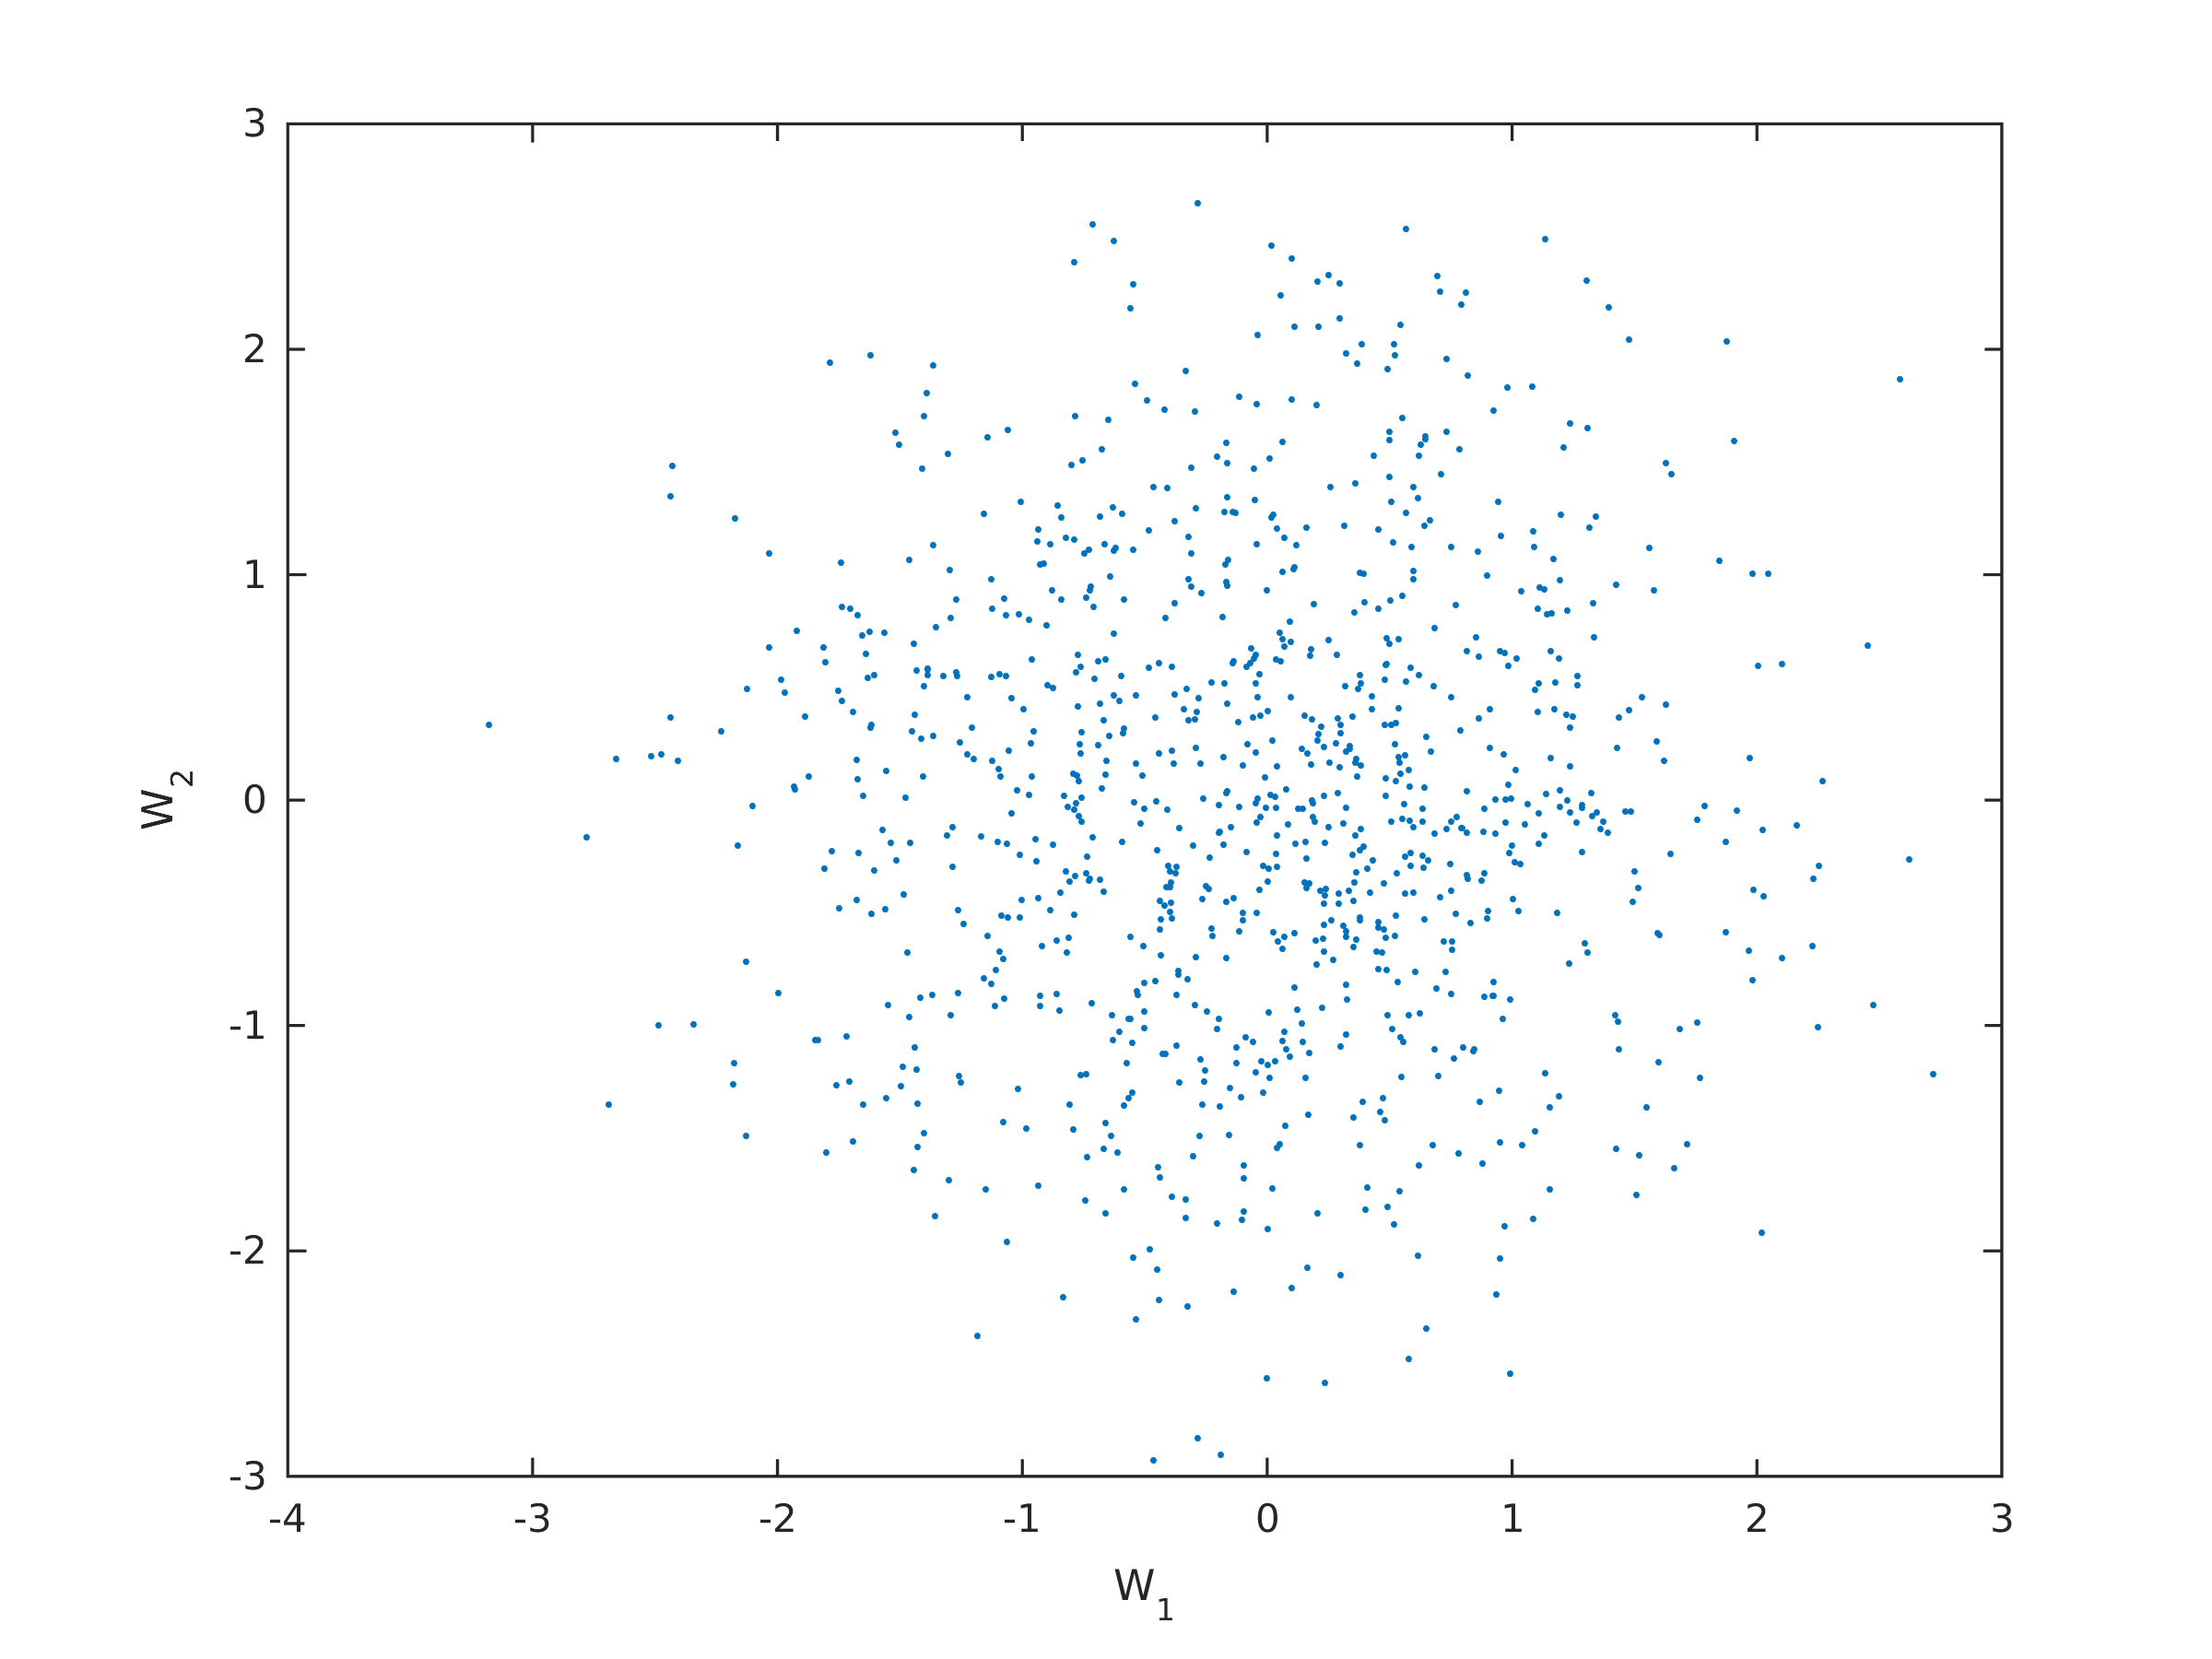
\includegraphics[width=0.5\textwidth]{rvW.png}
		\caption{Scatter plot for $W$}
		\end{center}
	\end{figure}
	\begin{figure}[h]
		\begin{center}
		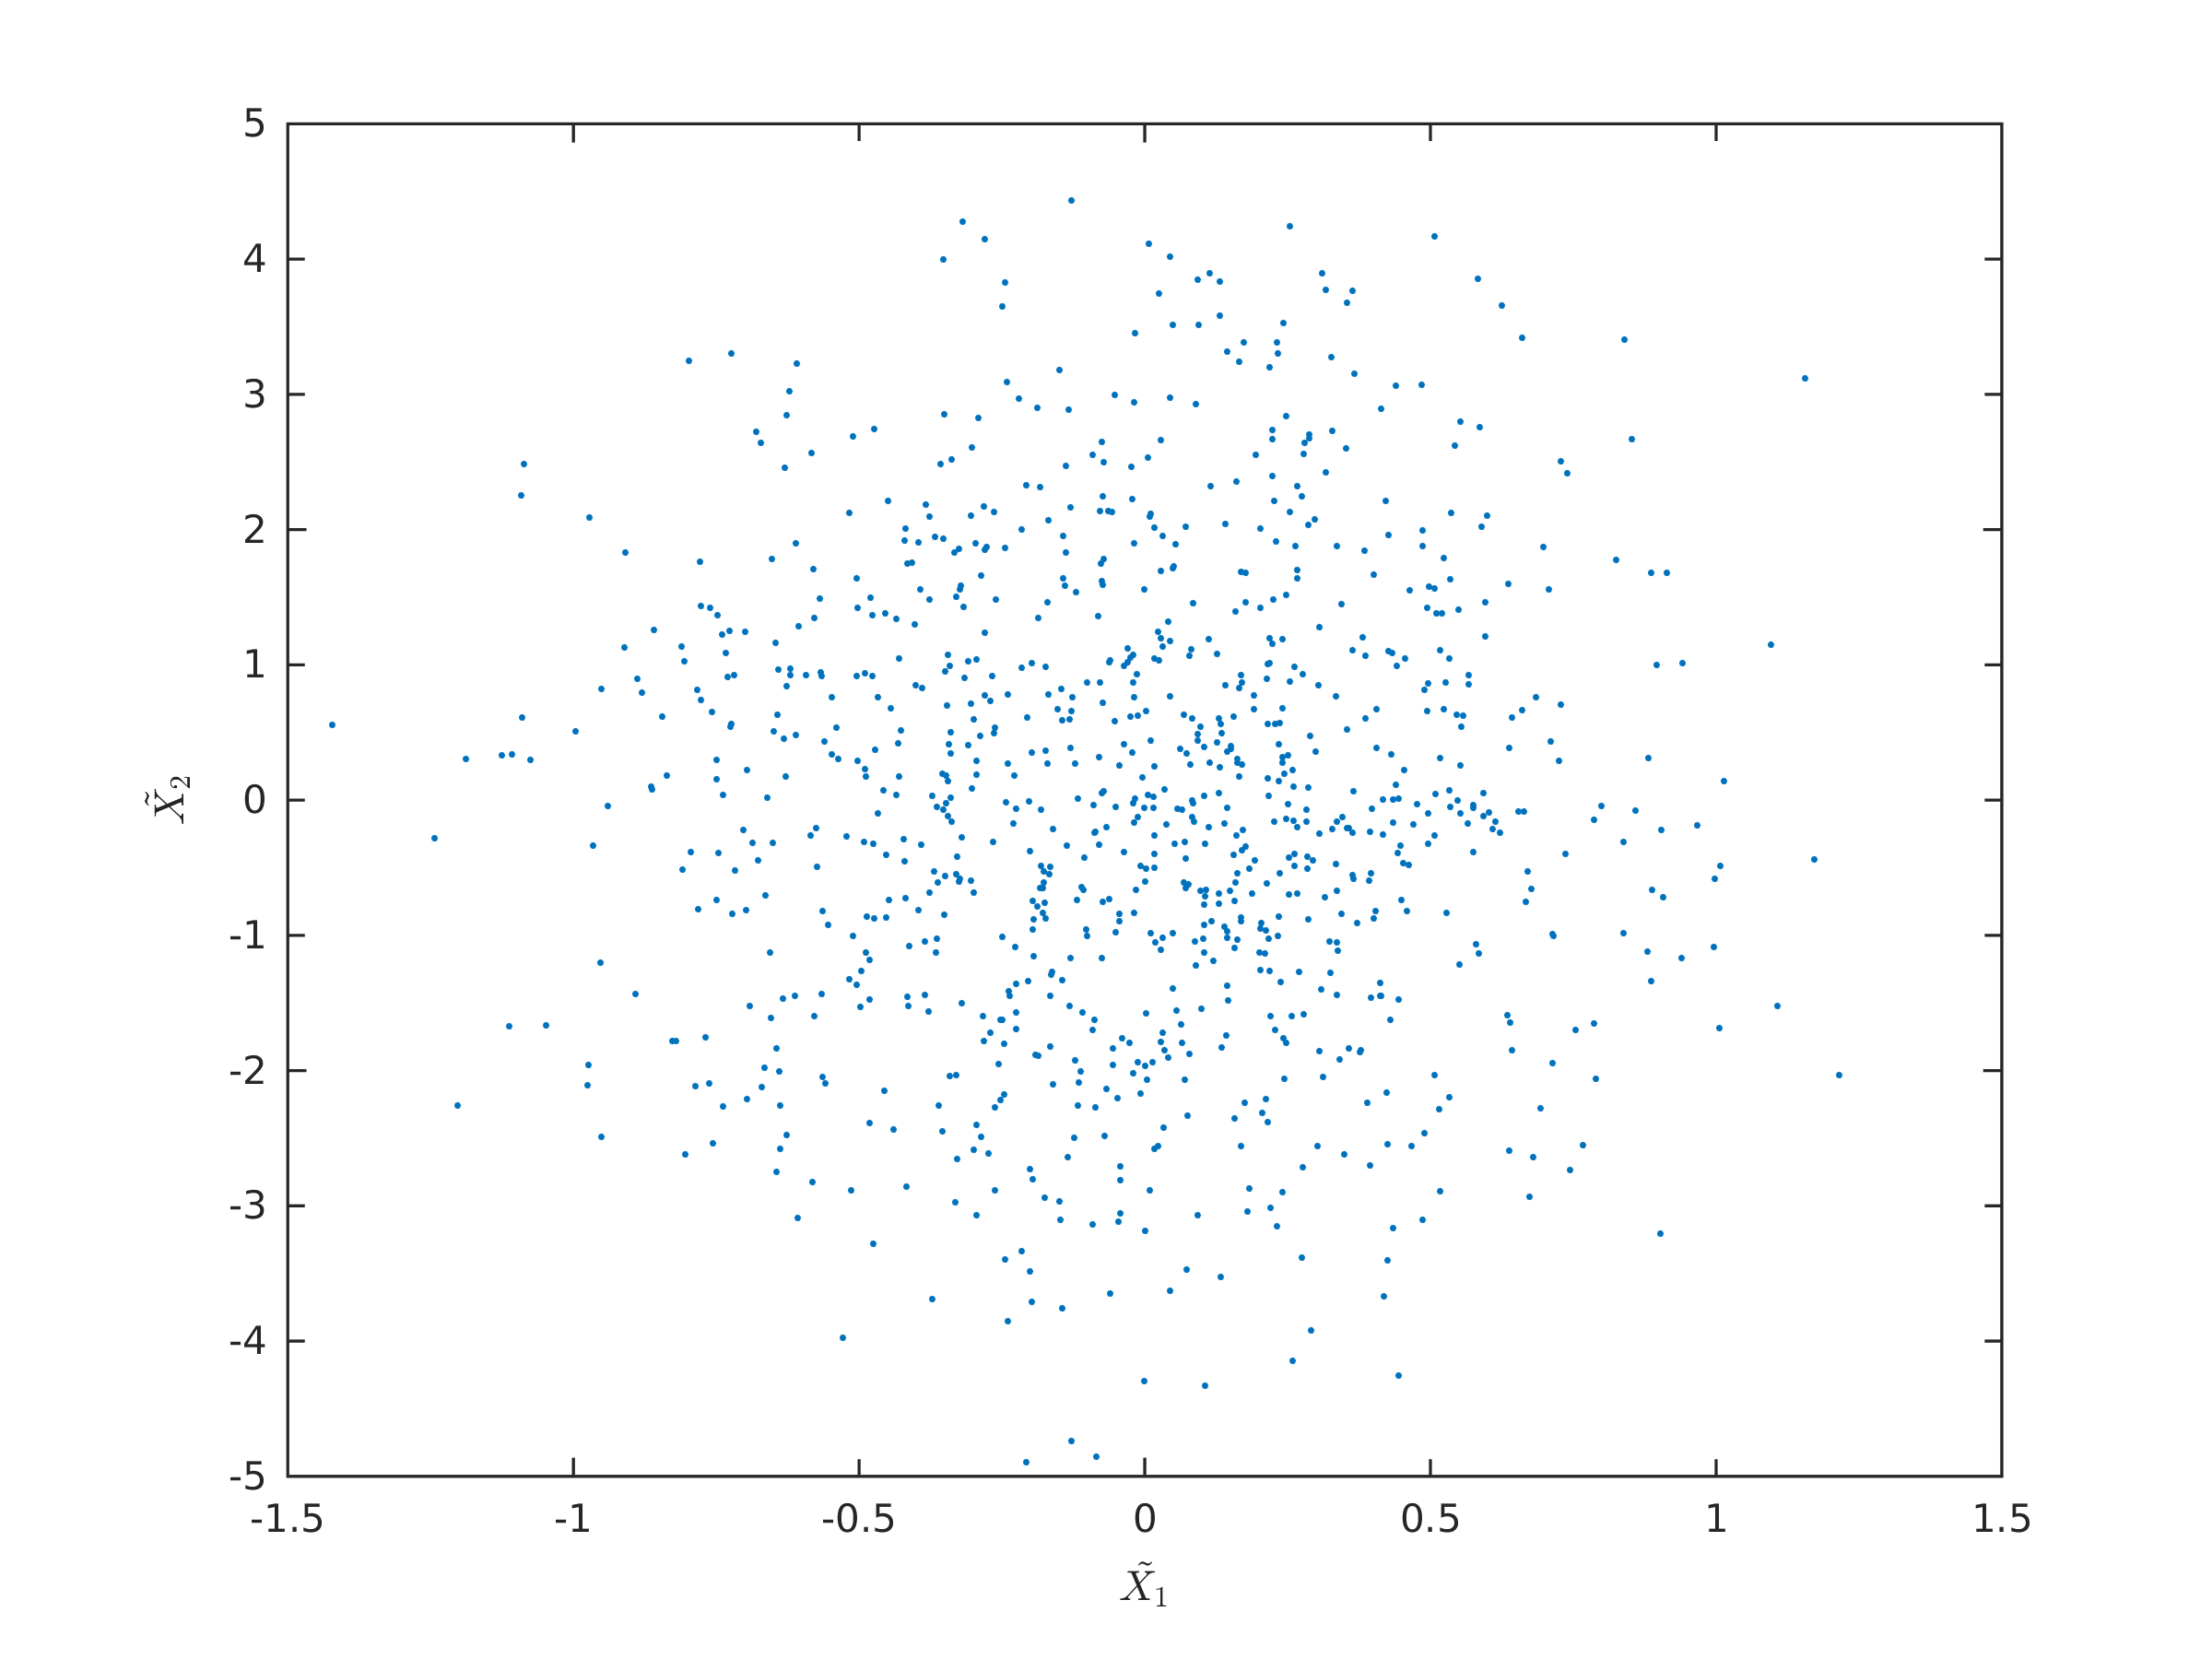
\includegraphics[width=0.5\textwidth]{rvXtilda.png}
		\caption{Scatter plot for $\tilde{X}$}
		\end{center}
	\end{figure}
	\begin{figure}[h]
		\begin{center}
		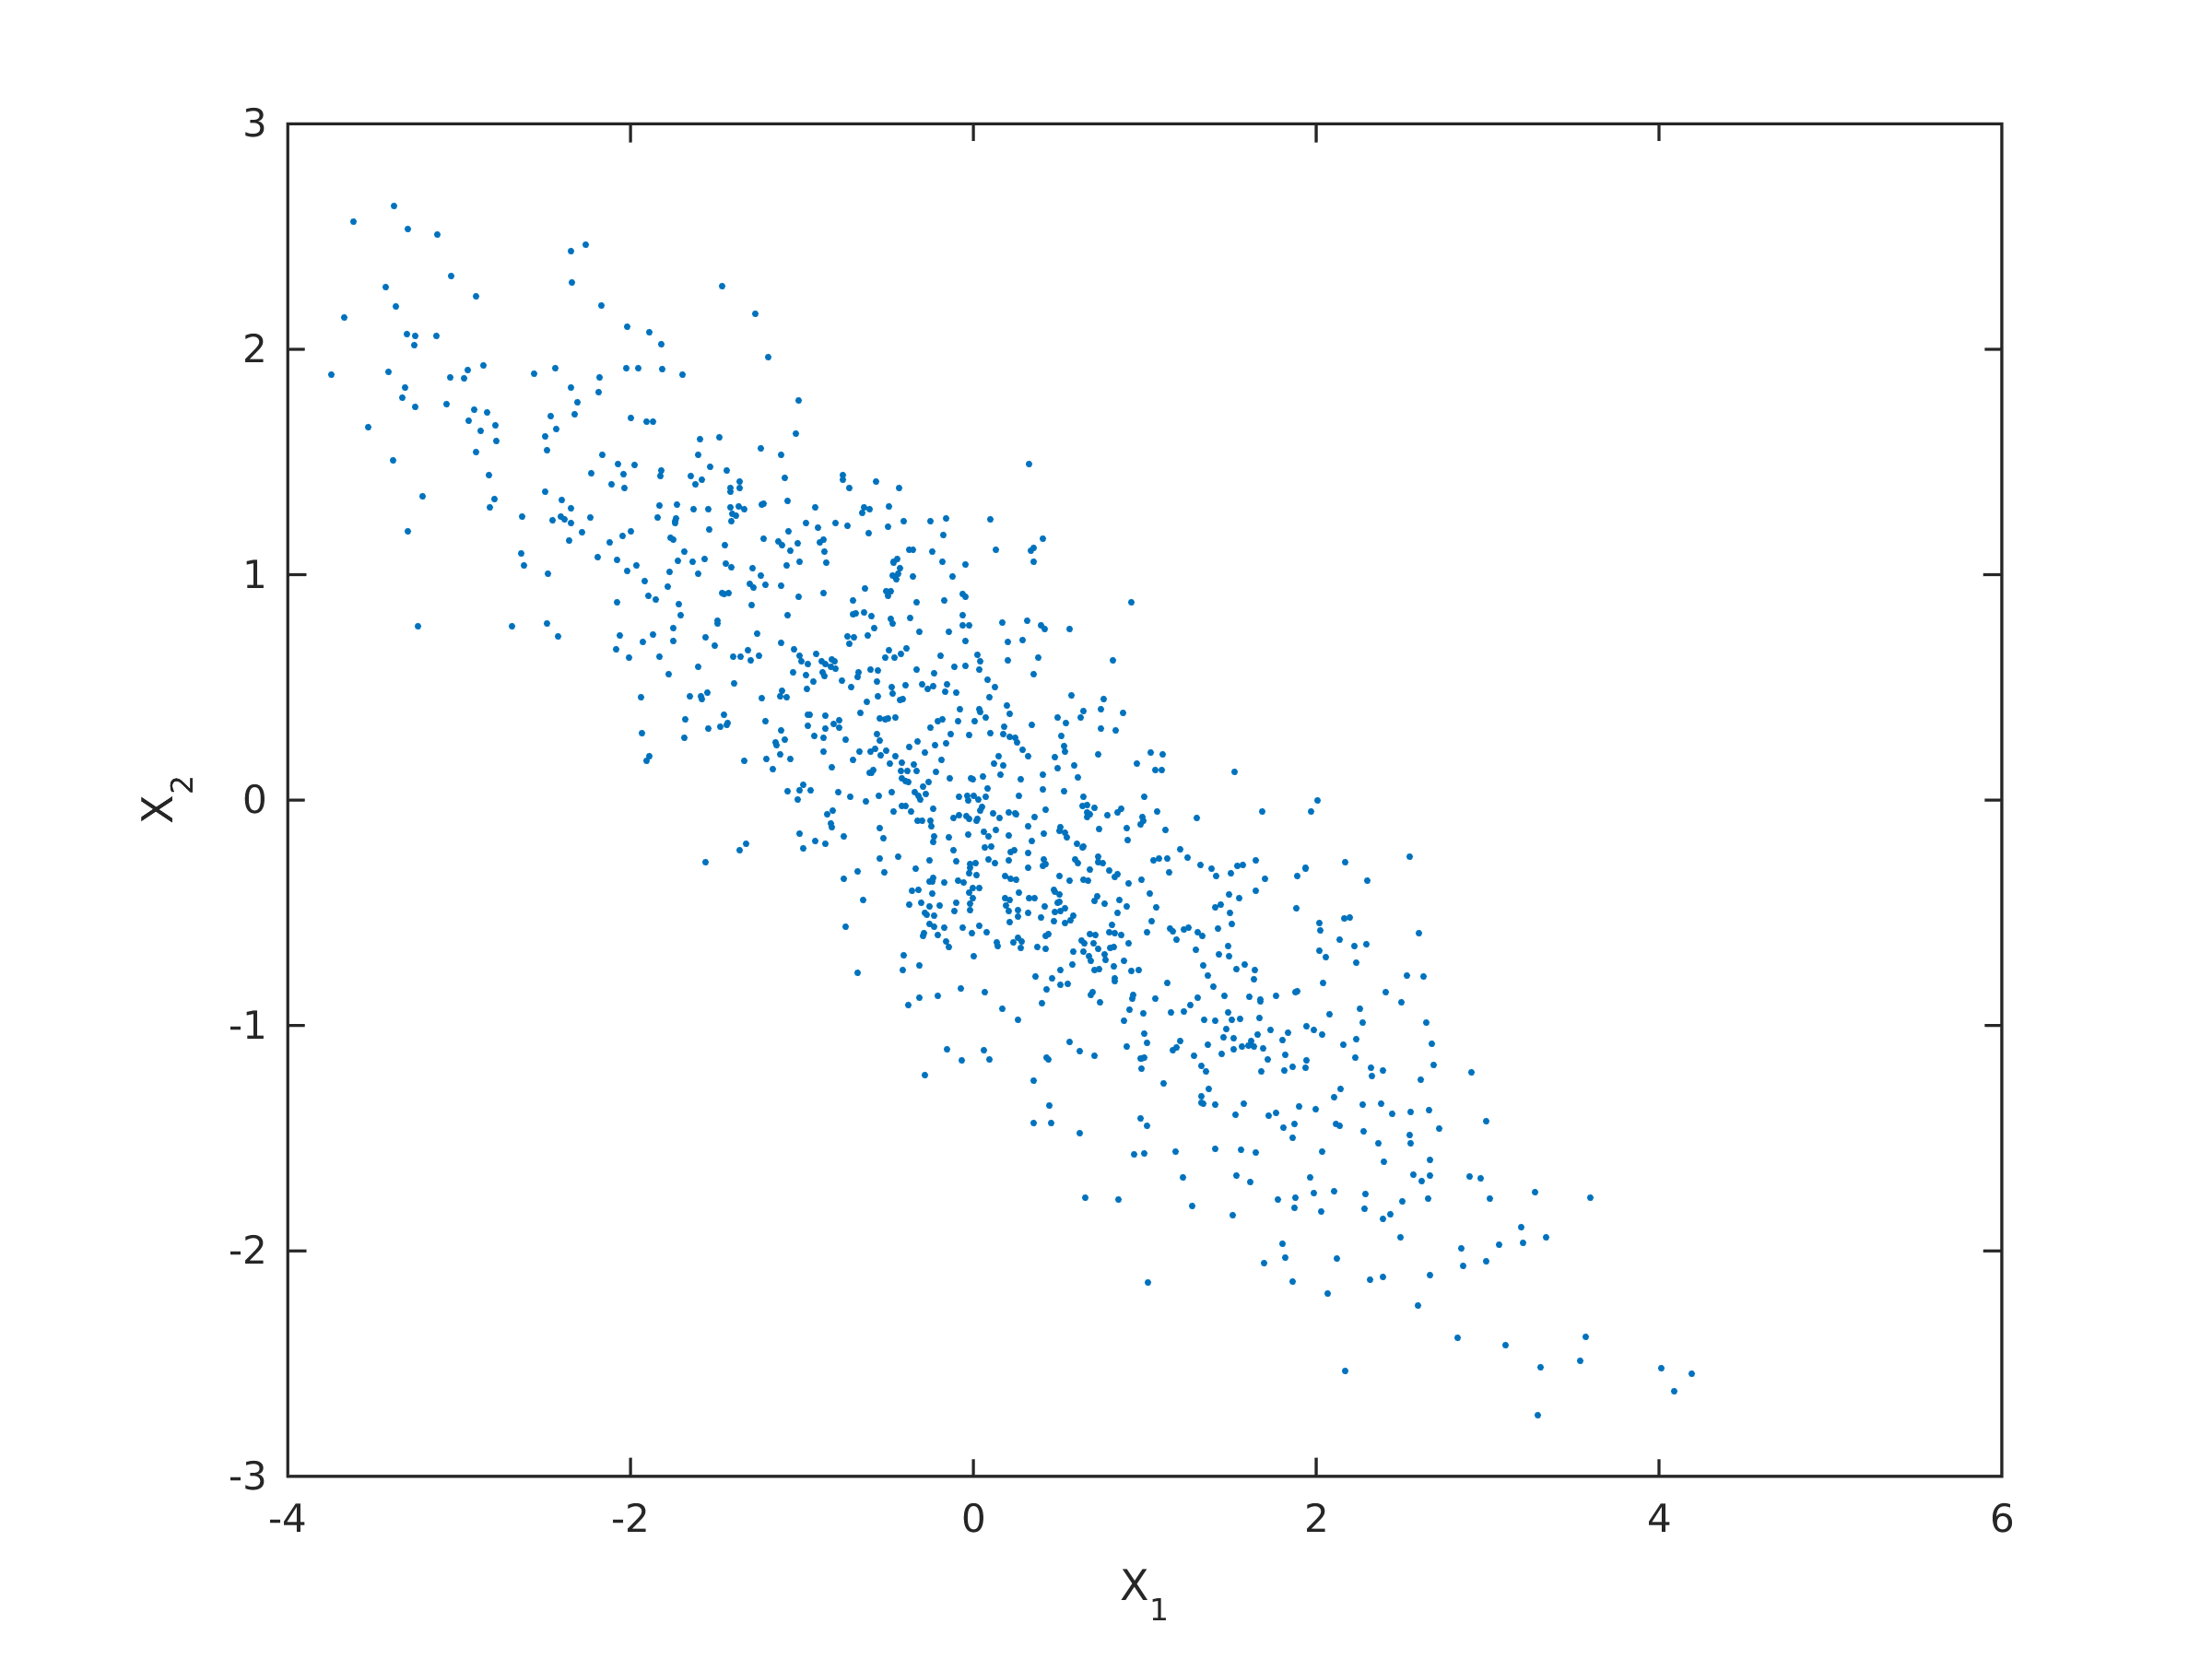
\includegraphics[width=0.5\textwidth]{rvX.png}
		\caption{Scatter plot for $X$}
		\end{center}
	\end{figure}

\pagebreak

	\subsection{Covariance Estimation and Whitening}
		\subsubsection{Theoretical Value of $R_{x}$}
			\begin{align*}
				R_{x} =
				\begin{bmatrix}
					2 & -1.2 \\
					-1.2 & 1
				\end{bmatrix}
			\end{align*}
		\subsubsection{Estimated Value of $\hat{R_{x}}$}
			\begin{align*}
				\hat{R_{x}} =
				\begin{bmatrix}
					2.0383 & -1.2230 \\
					-1.2230 & 1.0133
				\end{bmatrix}
			\end{align*}
		\subsubsection{Scatter Plots for $\tilde{X_{i}}$ and $W_{i}$}
			\begin{figure}[h]
				\begin{subfigure}{0.5\textwidth}
					\begin{center}
					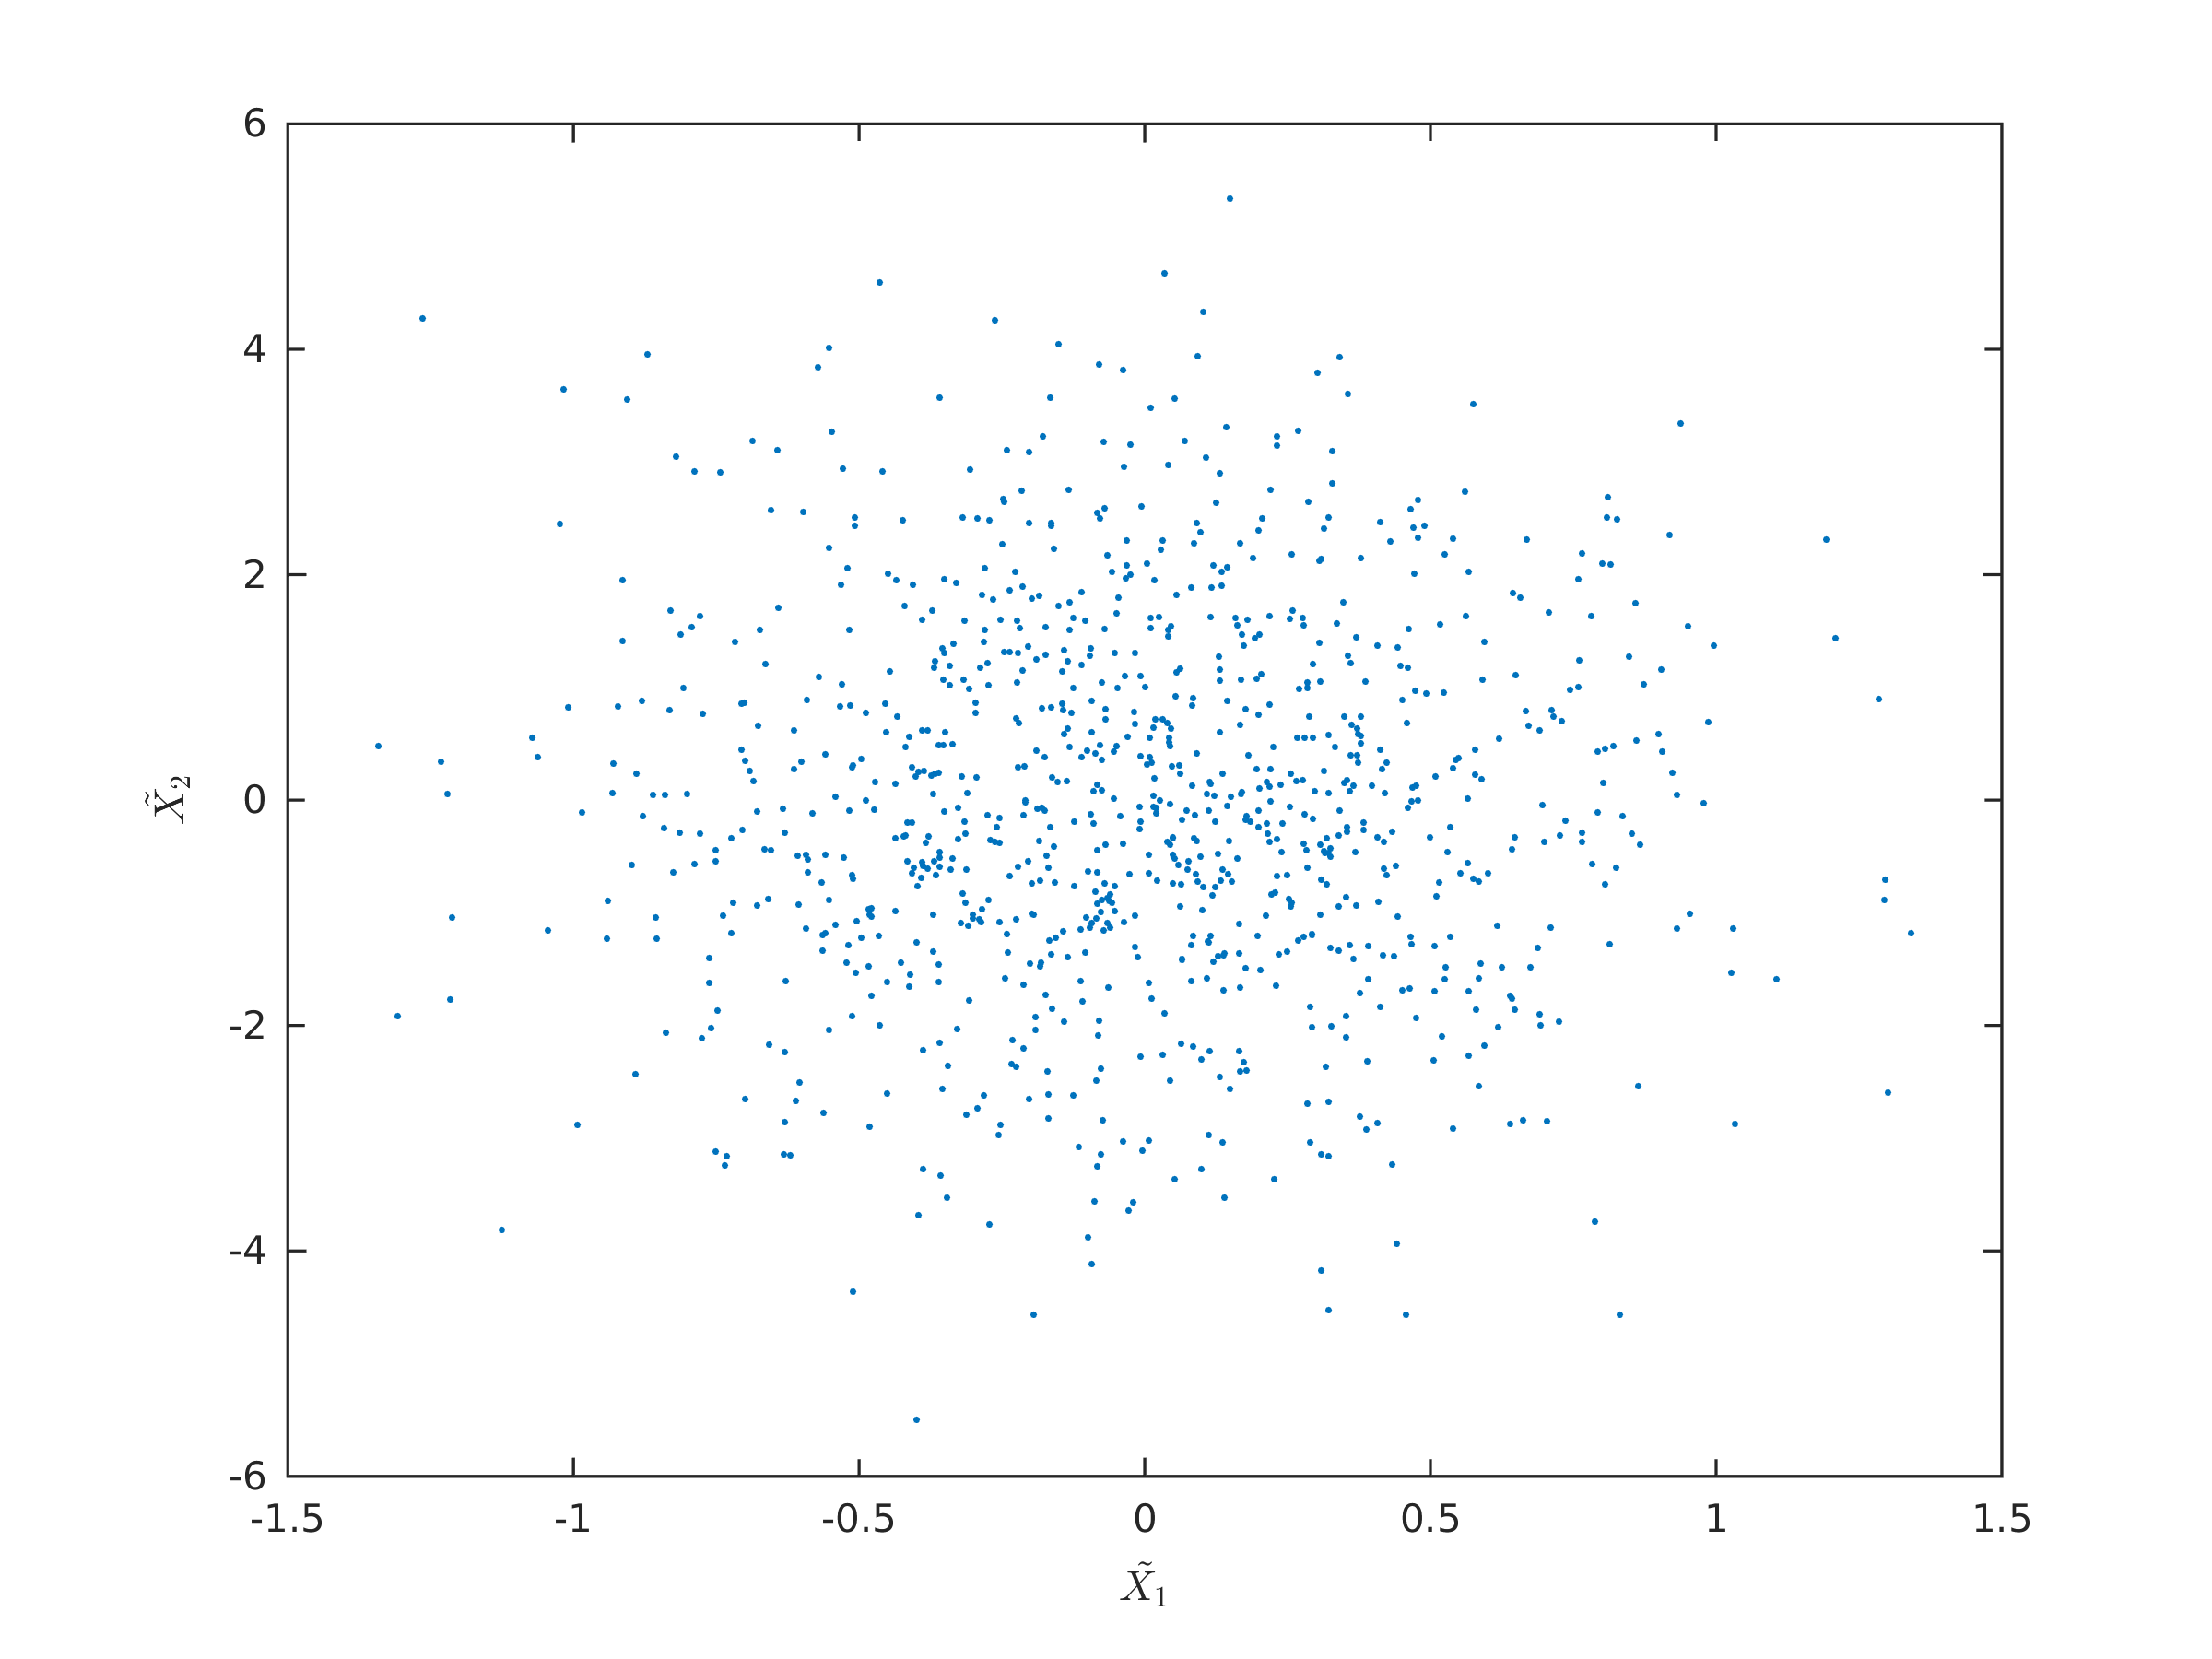
\includegraphics[width=0.8\textwidth]{rvXtildaEsti.png}
					\caption{Scatter plot for $\tilde{X_{i}}$}
					\end{center}
				\end{subfigure}
				\begin{subfigure}{0.5\textwidth}
					\begin{center}
					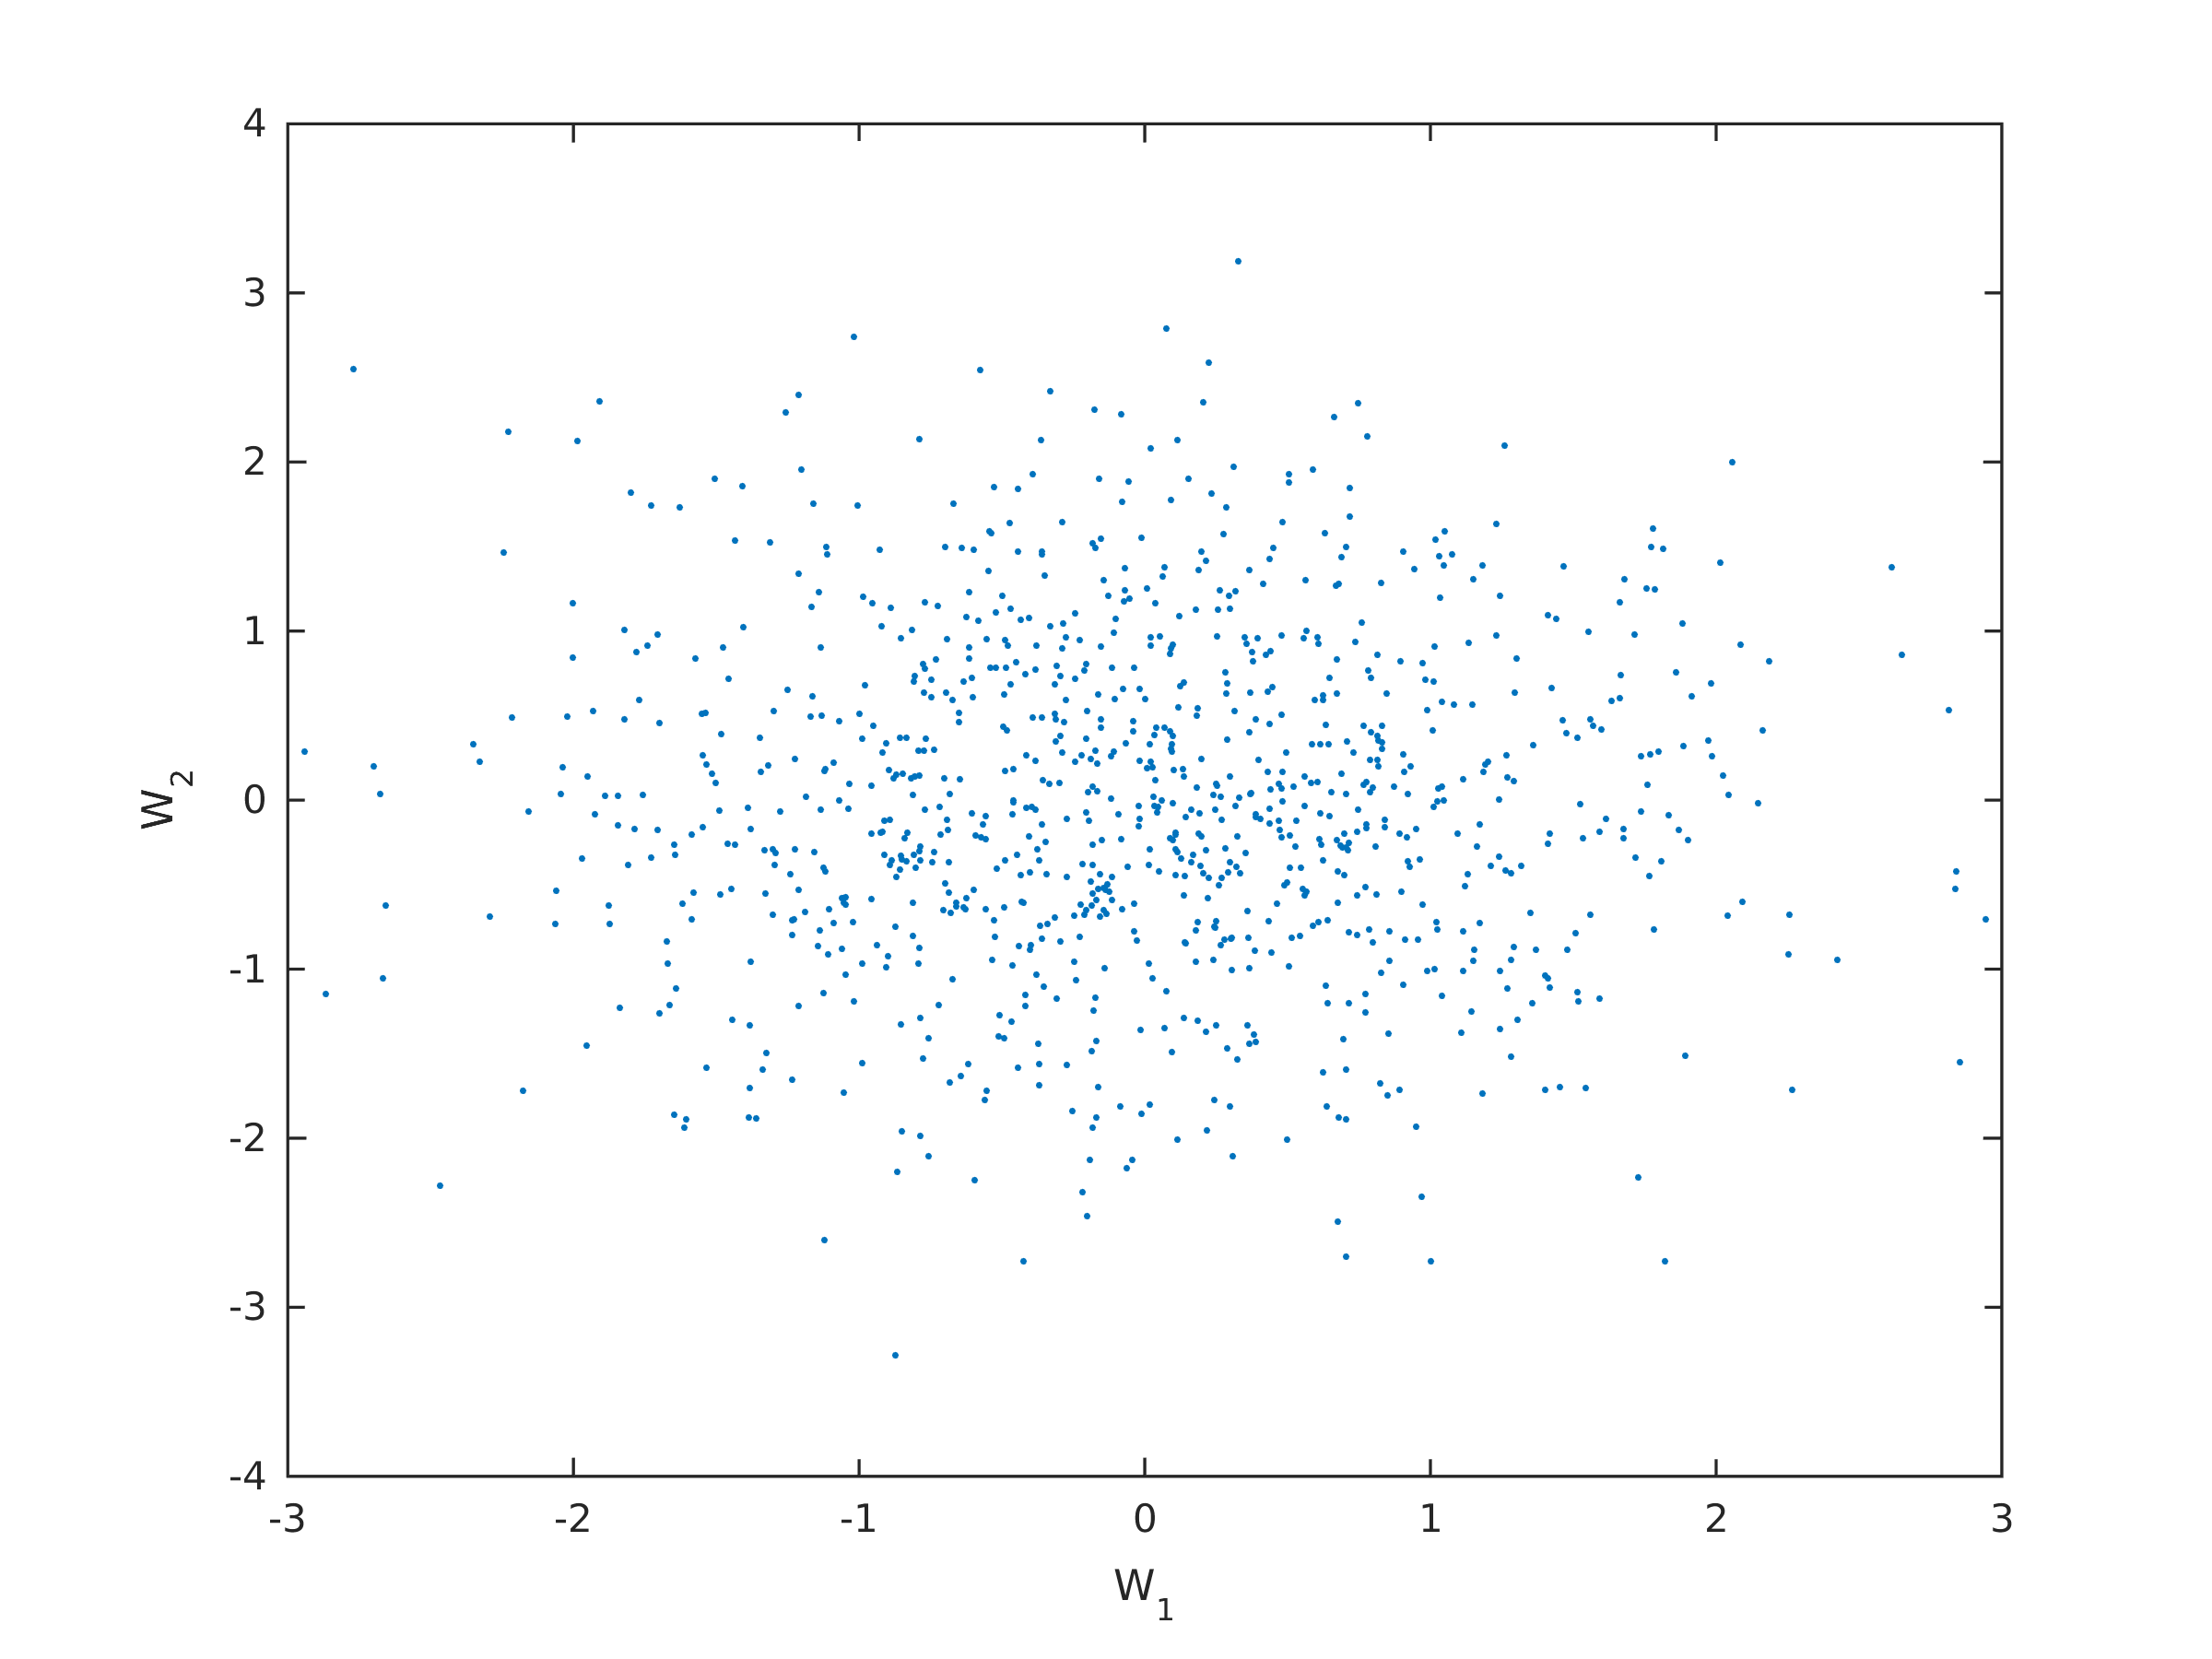
\includegraphics[width=0.8\textwidth]{rvWEsti.png}
					\caption{Scatter plot for $W_{i}$}
					\end{center}
				\end{subfigure}
			\end{figure}
		\subsubsection{Estimated Covariance of Whitened Process}
			\begin{align*}
				\hat{R_{W}} =
				\begin{bmatrix}
					1 & 0 \\
					0 & 1
				\end{bmatrix}
			\end{align*}

%----------------------------------------------------------------------------------------
%	SECTION 3
%----------------------------------------------------------------------------------------
\section{Estimation of Eigenvectors and Eigenvalues Using the Signular Value
Decomposition}

Nothing due for report.

%----------------------------------------------------------------------------------------
%	SECTION 4
%----------------------------------------------------------------------------------------
\section{Eigenimages, PCA and Data Reduction}
	\subsection{12 Eigenvalues}
		\begin{figure}[h]
			\begin{center}
				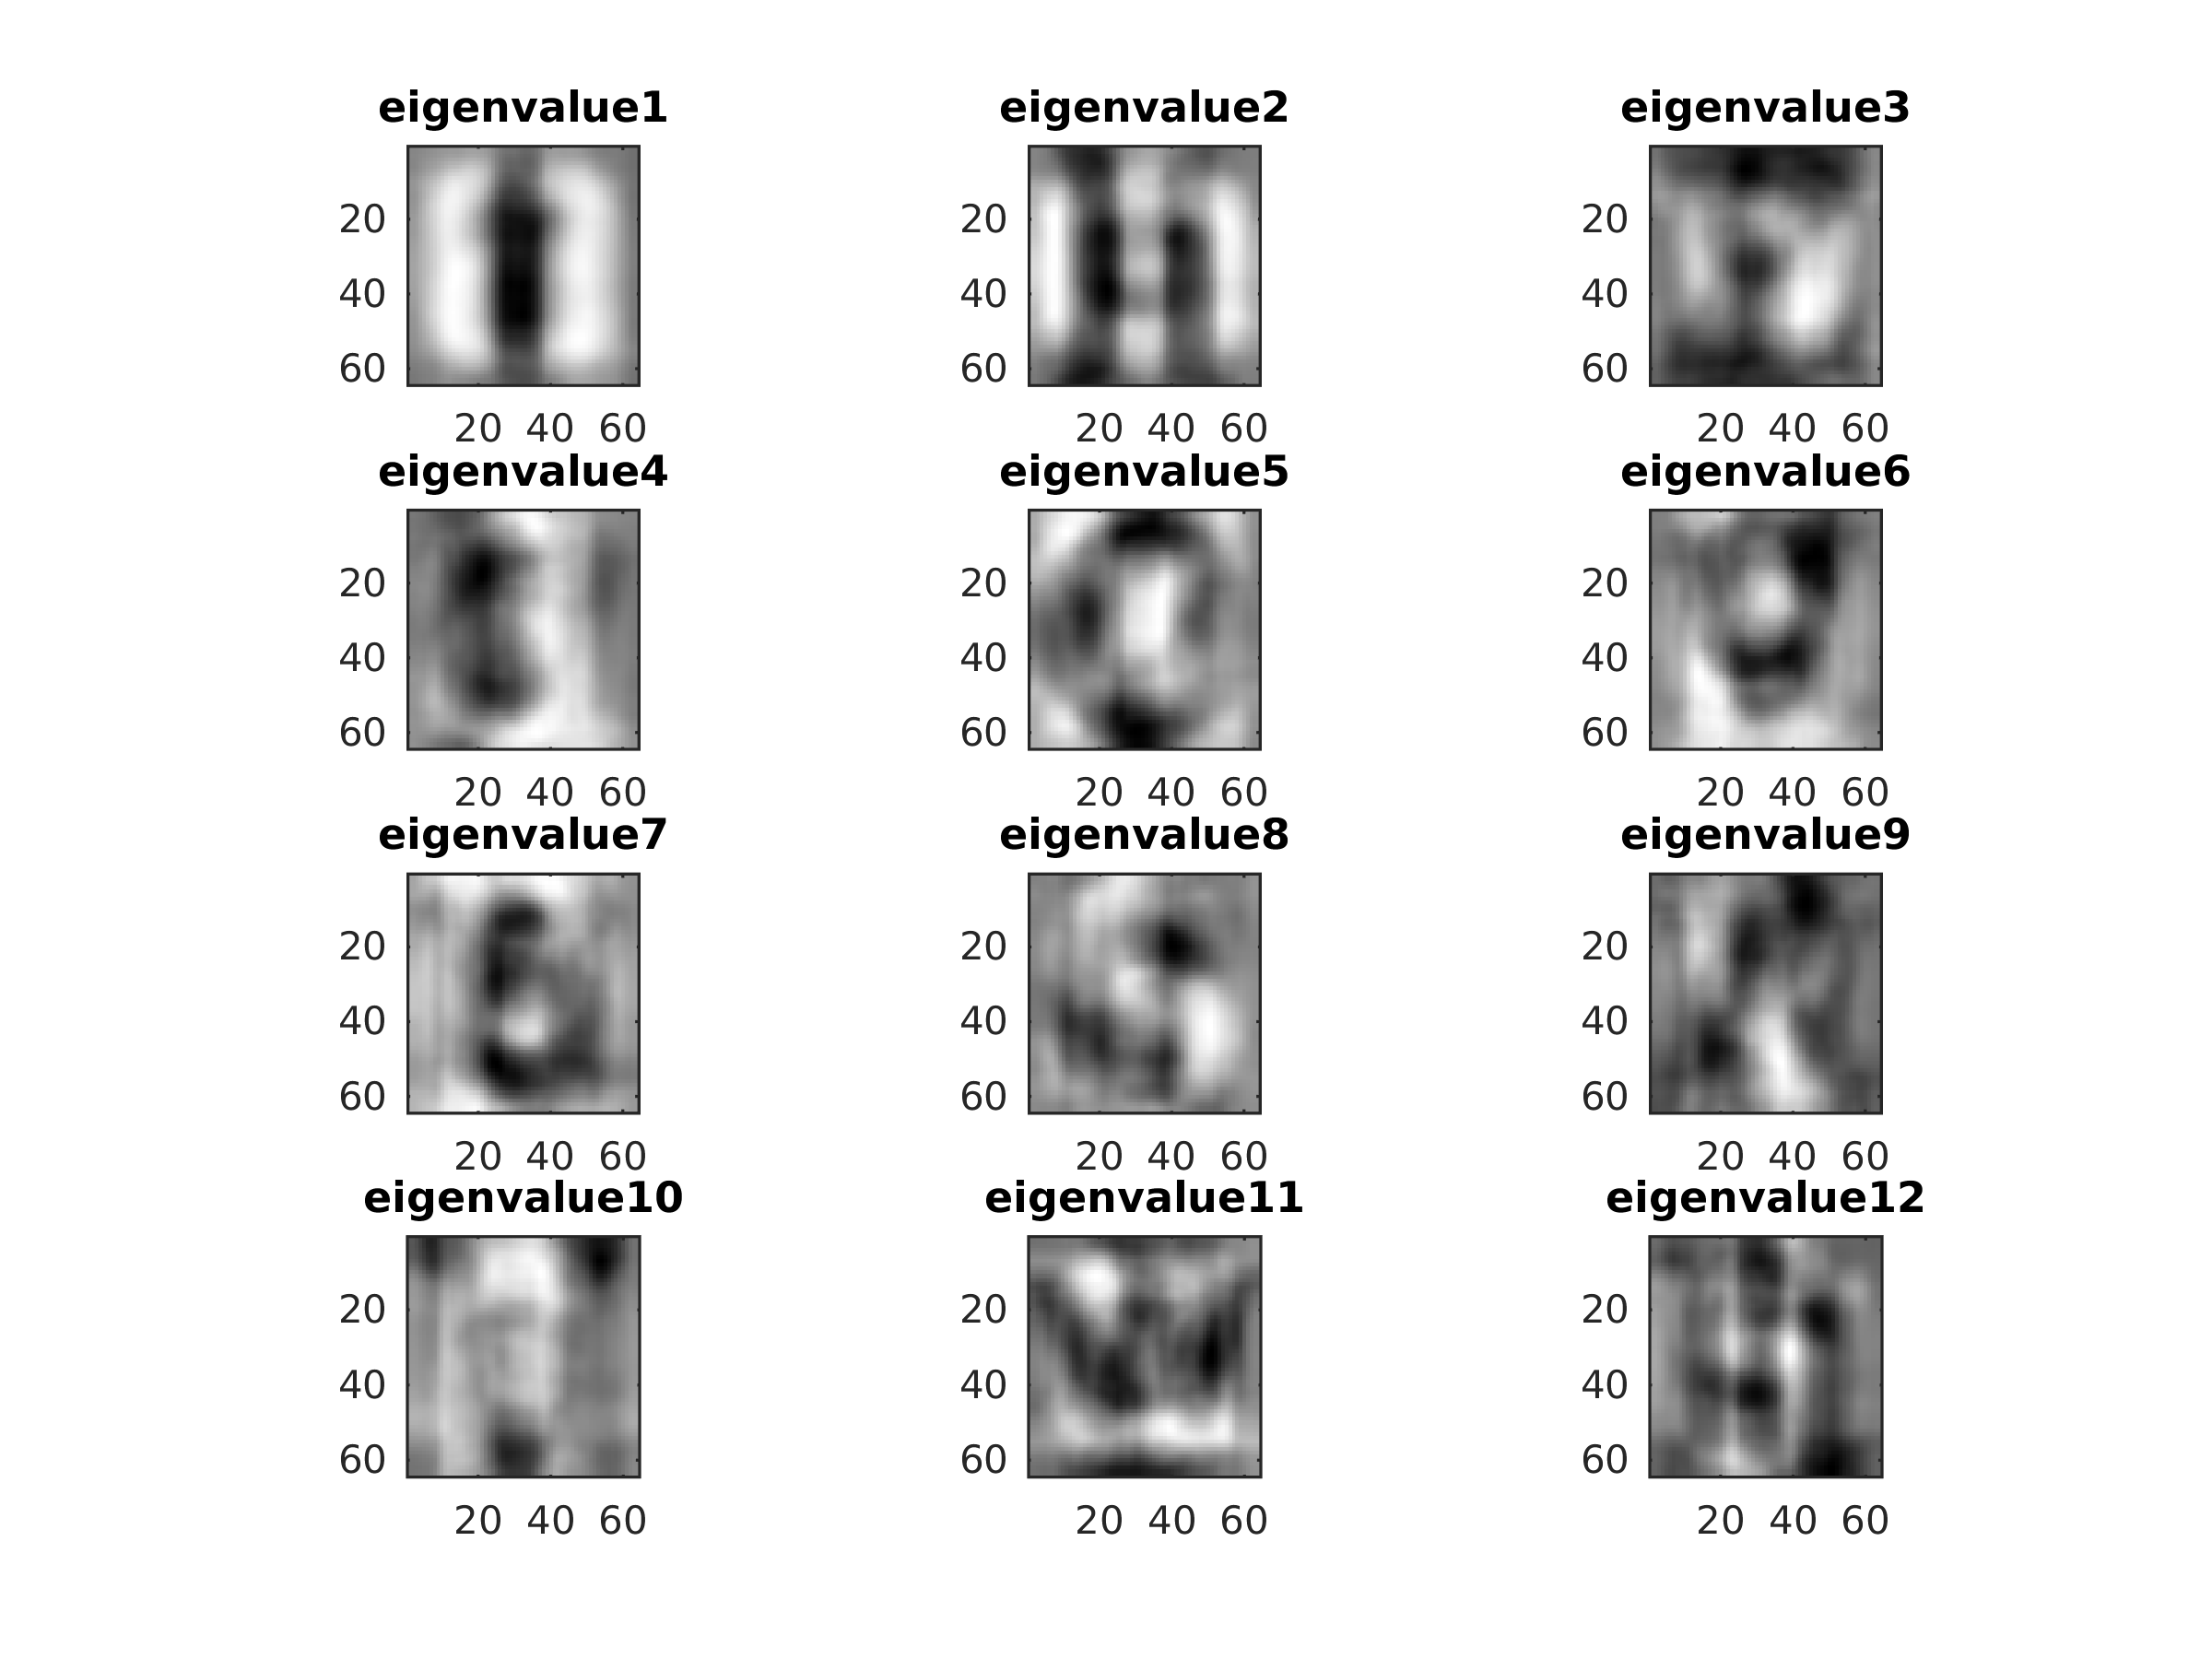
\includegraphics[width=0.6\textwidth]{12eigimgs.png}
				\caption{12 Eigenimages}
			\end{center}
		\end{figure}
	\subsection{Projection Coefficients vs. Eigenvector Number}
		\begin{figure}[h]
			\begin{center}
				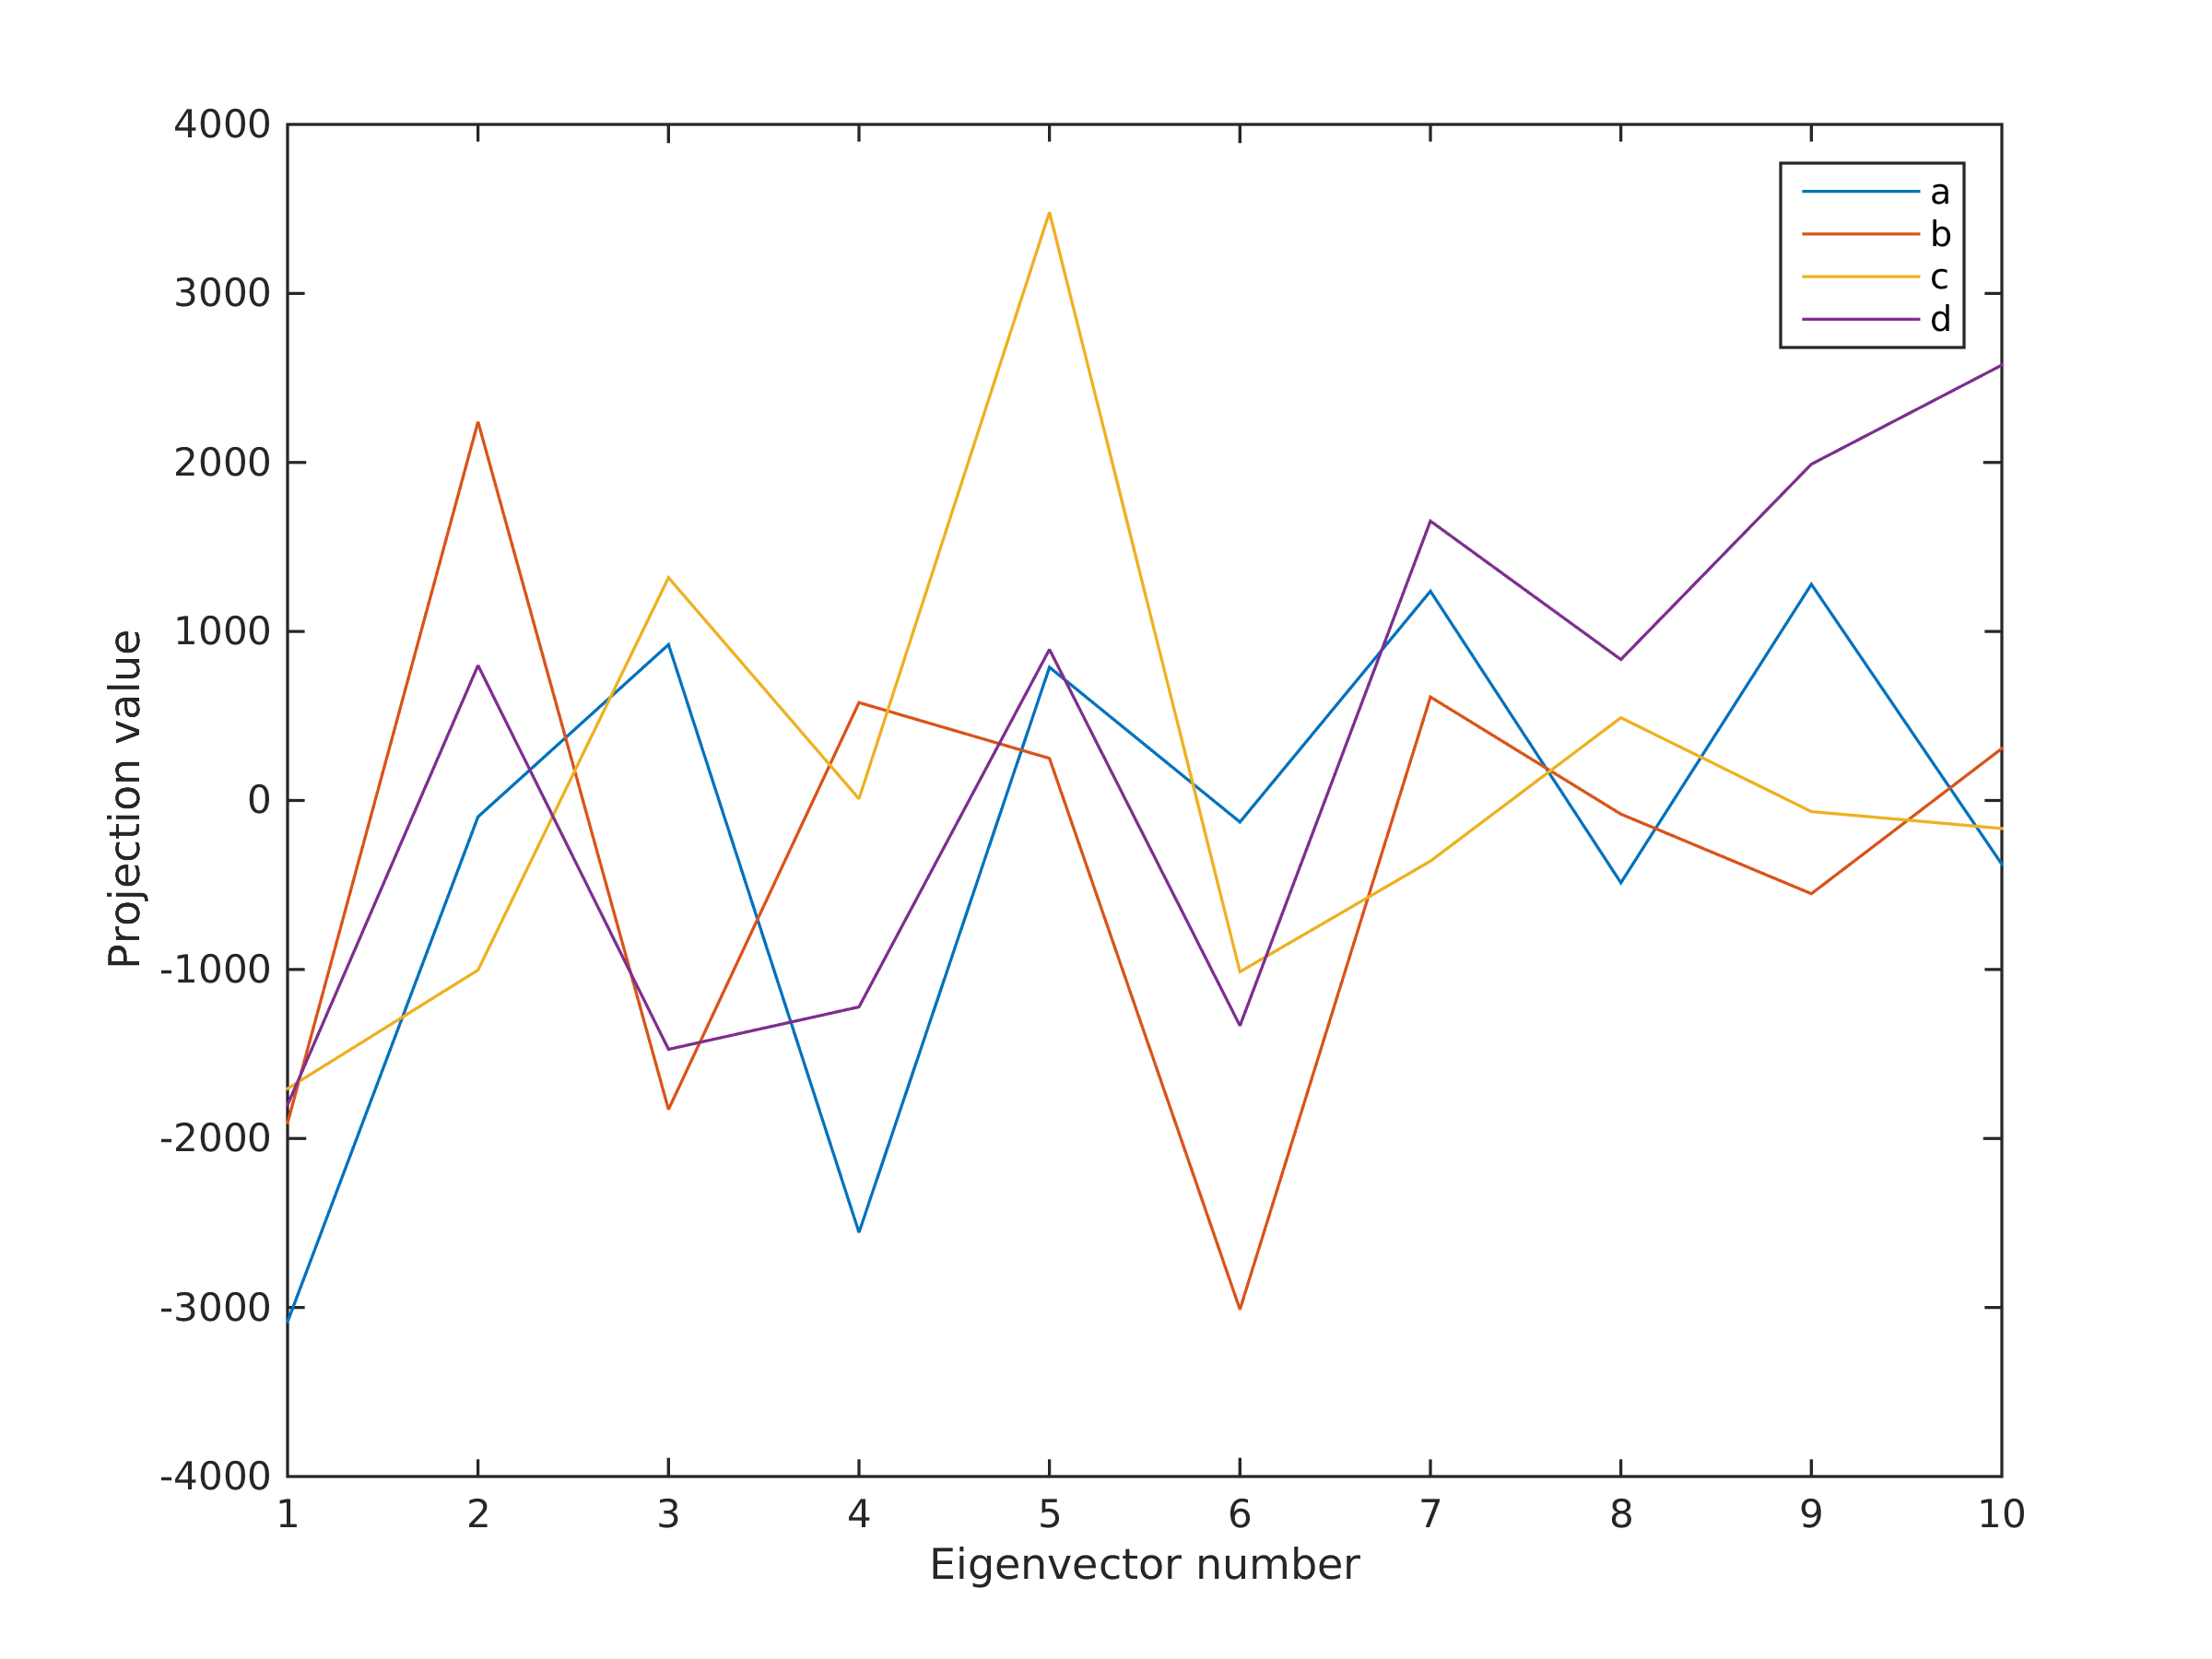
\includegraphics[width=0.6\textwidth]{projCoefVseigNum.png}
				\caption{Projection Coefficients vs. Eigenvector Number}
			\end{center}
		\end{figure}
	\subsection{Original Image and the 6 Resynthesized Images}
		\begin{figure}[h]
			\begin{center}
				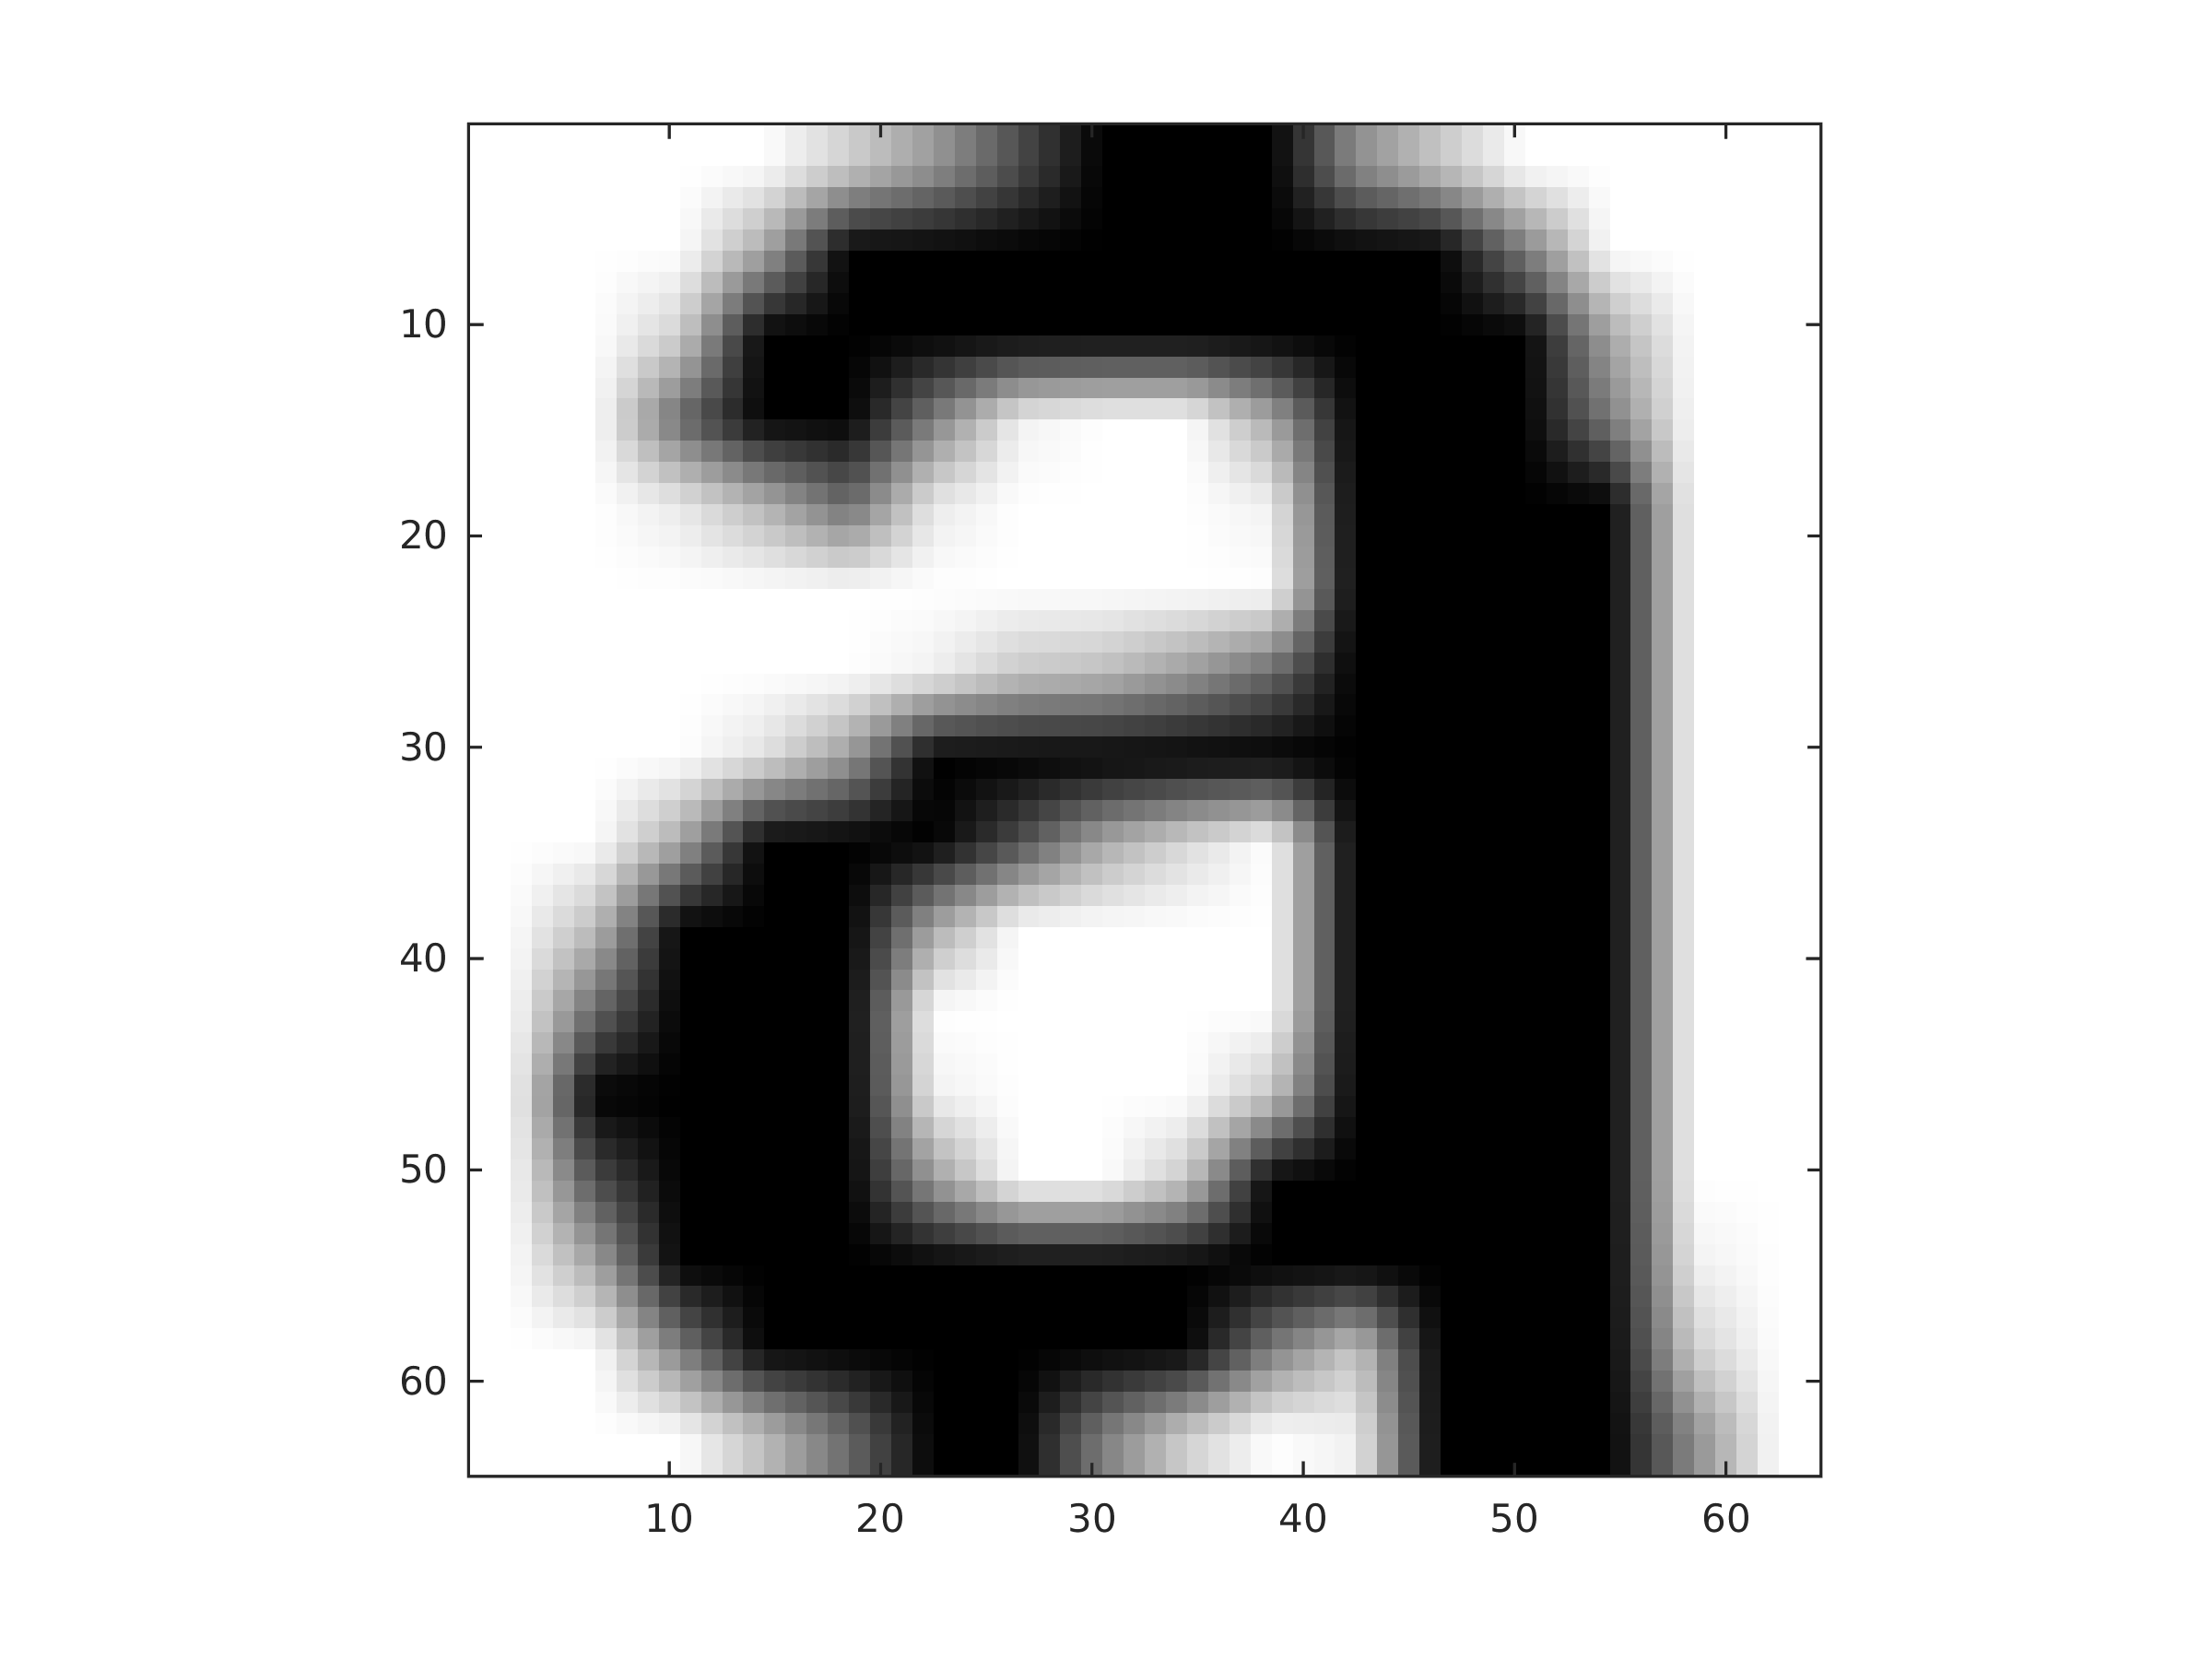
\includegraphics[width=0.6\textwidth]{orgA.png}
				\caption{The Original Image of "a"}
			\end{center}
		\end{figure}

\pagebreak

		\begin{figure}[h]
			\begin{center}
				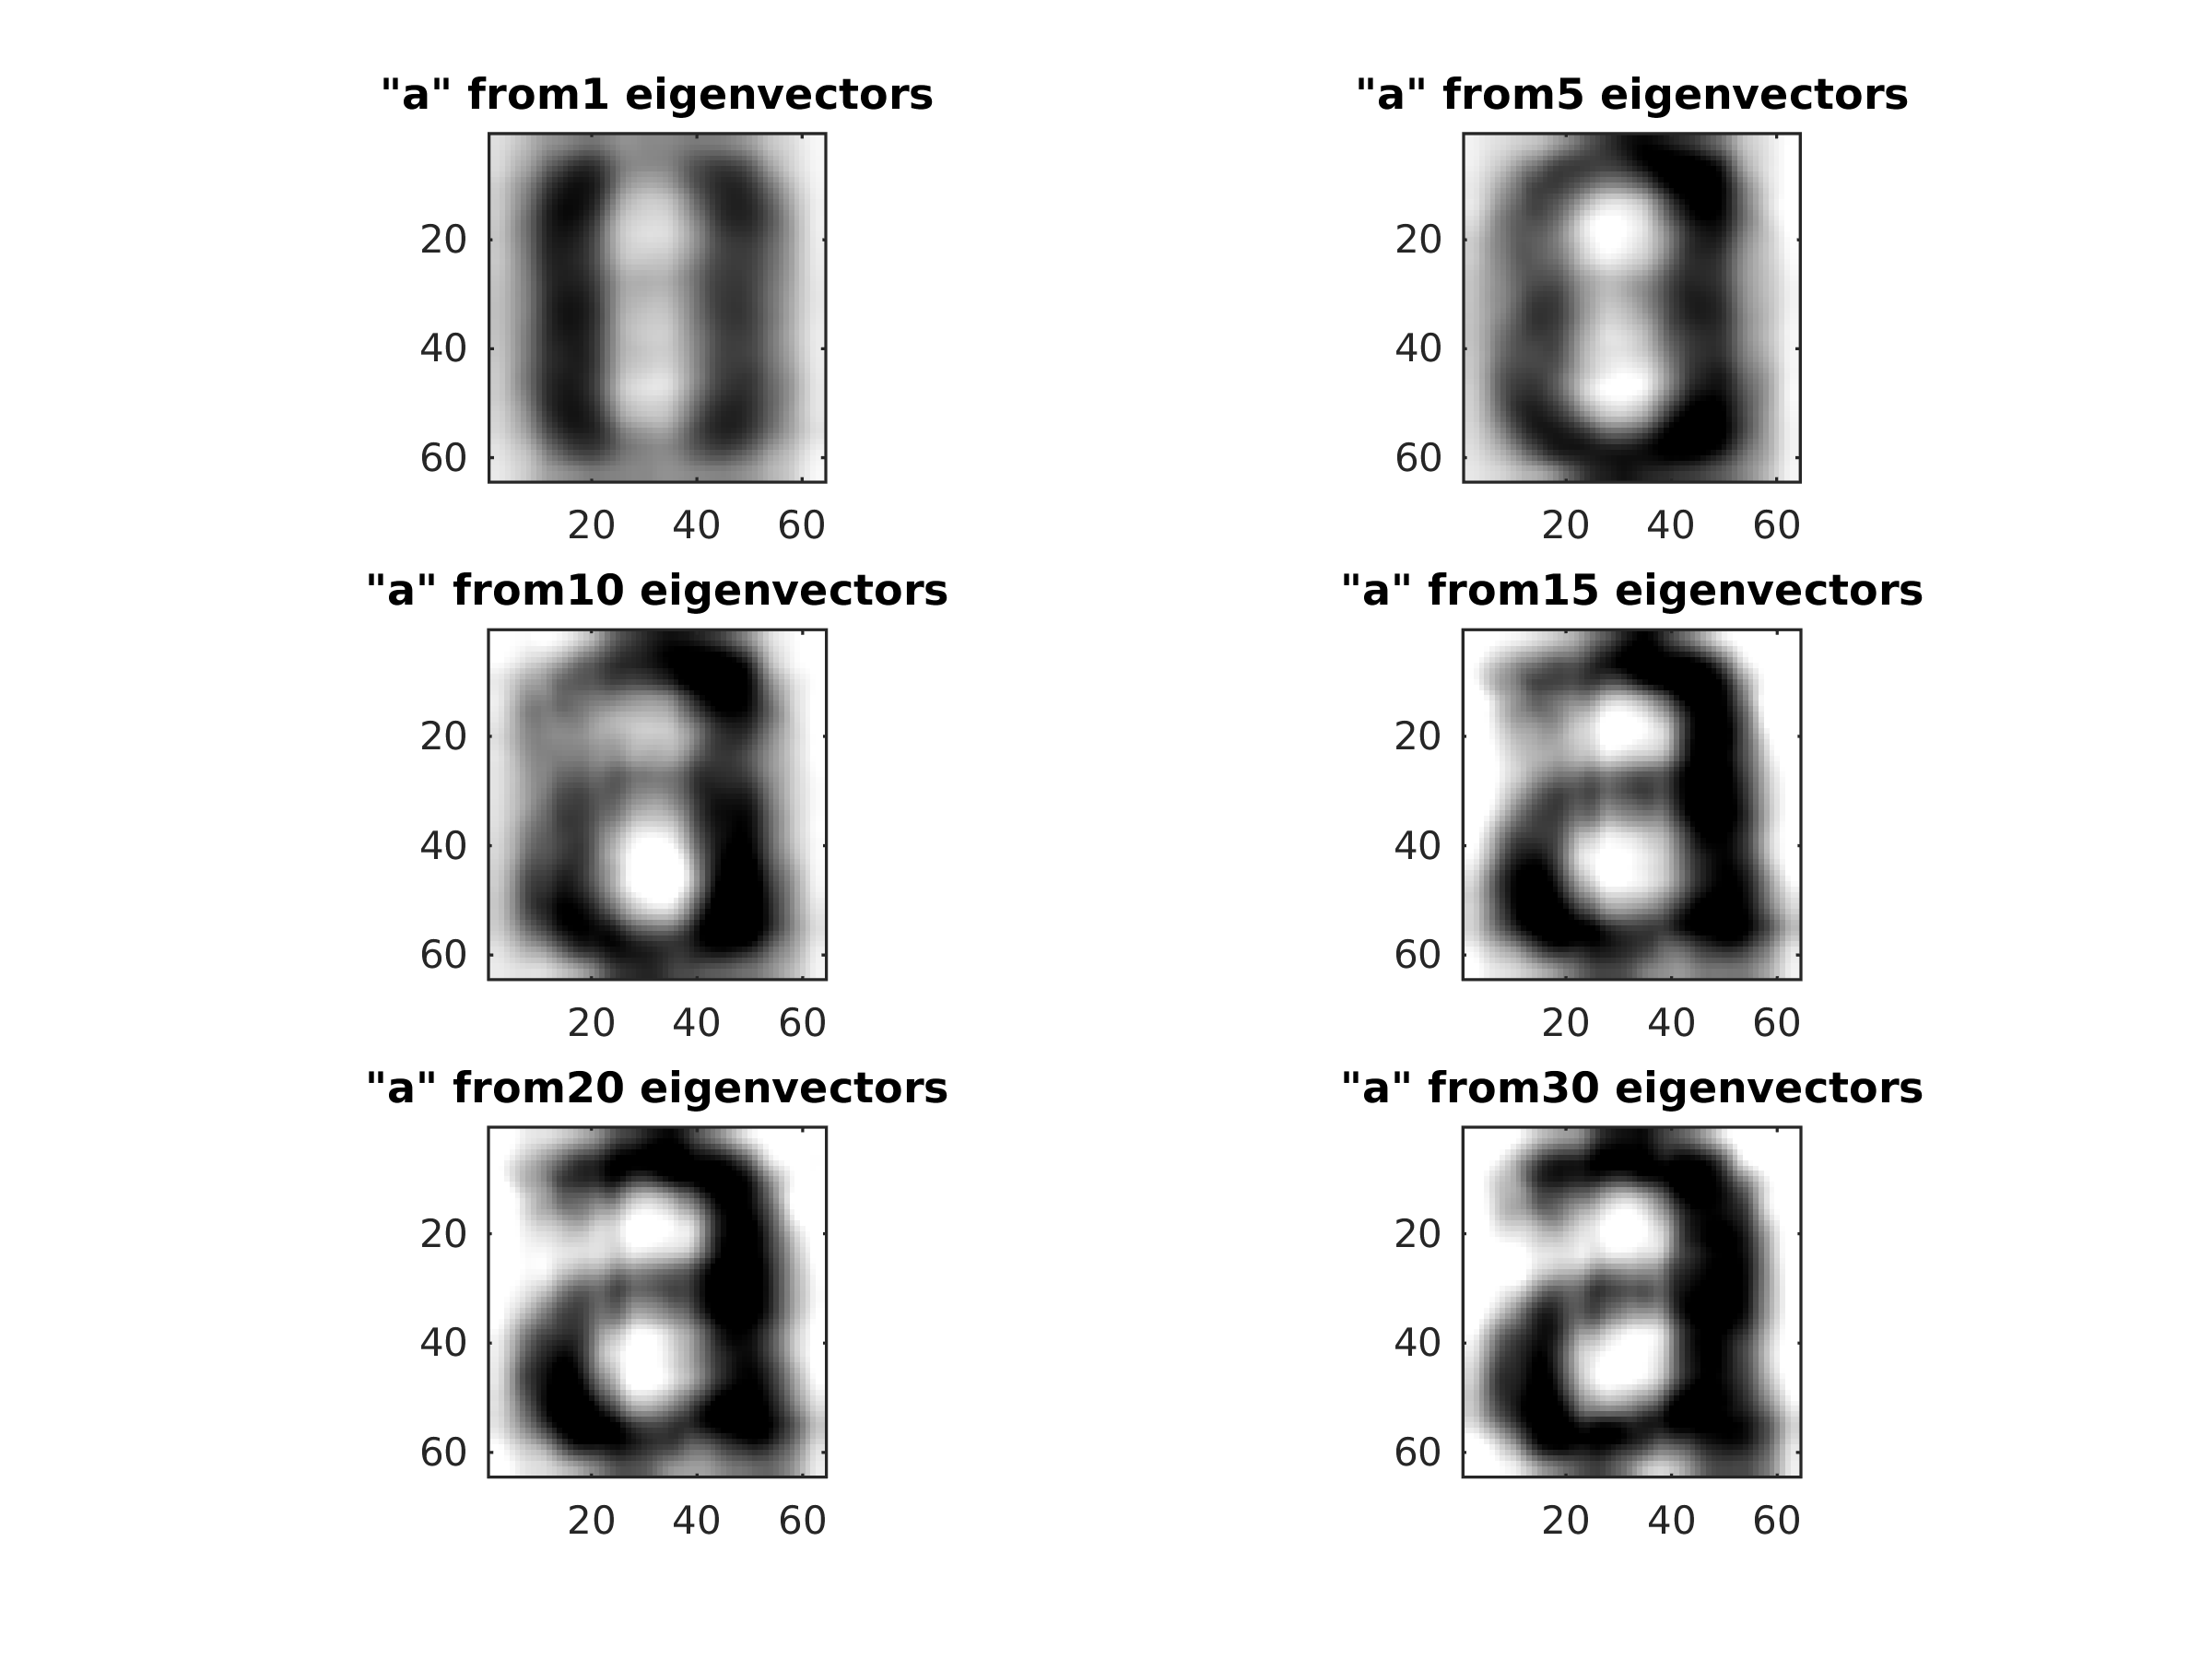
\includegraphics[width=0.6\textwidth]{synA.png}
				\caption{Synthesized Versions of of "a"}
			\end{center}
		\end{figure}

%----------------------------------------------------------------------------------------
%	SECTION 5
%----------------------------------------------------------------------------------------

\section{Image Classification}
	\subsection{Classification and PCA}
		\subsubsection{Classification errors using Eigenvectors}
			\begin{center}
				\begin{tabular}{| l | c |}
					\hline
					Acutual Letter & Mis-classified Letter \\ \hline
					d & a \\ \hline
					j & y \\ \hline
					l & i \\ \hline
					n & v \\ \hline
					p & e \\ \hline
					q & a \\ \hline
					u & a \\ \hline
					y & v \\ \hline
				\end{tabular}
			\end{center}
		\subsubsection{Classification errors using $B_{k}=\Lambda_{k}$}
			\begin{center}
				\begin{tabular}{| l | c |}
					\hline
					Acutual Letter & Mis-classified Letter \\ \hline
					i & l \\ \hline
					y & v \\ \hline
				\end{tabular}
			\end{center}
		\subsubsection{Classification errors using $B_{k}=R_{wc}$}
			\begin{center}
				\begin{tabular}{| l | c |}
					\hline
					Acutual Letter & Mis-classified Letter \\ \hline
					g & q \\ \hline
					y & v \\ \hline
				\end{tabular}
			\end{center}
		\subsubsection{Classification errors using $B_{k}=\Lambda$}
			\begin{center}
				\begin{tabular}{| l | c |}
					\hline
					Acutual Letter & Mis-classified Letter \\ \hline
					f & t \\ \hline
					y & v \\ \hline
				\end{tabular}
			\end{center}
		\subsubsection{Classification errors using $B_{k}=I$}
			\begin{center}
				\begin{tabular}{| l | c |}
					\hline
					Acutual Letter & Mis-classified Letter \\ \hline
					f & t \\ \hline
					g & q \\ \hline
					y & v \\ \hline
				\end{tabular}
			\end{center}
	\subsection{Conclusions}
		1. $B_k=\Lambda_k$,$B_k=R_wc$, and $B_k=\Lambda$ have similar
		performance and have the smallest amount of errors. \\
		2. There is a trade-off between the data model accuracy and estimate
		accuracy. More complex the model is, poorer performance of the
		estimation accuracy.
\end{document}
